\section[Die Architektur der Applikation(Jürgen Hetzel)]{Android Grundlagen \begin{tiny} (Jürgen
Hetzel)\end{tiny}}Das Android-Framework enhält die folgenden vier grundlegenden Bausteine:
\begin{itemize}
   \item \textbf{Activities:}\\
   Activities sind Teilaspekte aus denen eine Applikation aufgebaut ist. Sie beinhalten
   üblicherweise Benutzerobefläche, Menü, Navigation und Programmlogik \cite[vgl.][S.
   89]{AppsProg}.
   \item \textbf{ContentProvider:}\\
   Mit Hilfe von \emph{ConentProvidern} ist es möglich, die Daten der eigenen Applikation
   anderen Anwendungen in Form von Tabellen zur Verfügung zu stellen \cite[vgl.][S. 212]{AppsProg}.
   \item \textbf{Services:}\\
   Die \emph{Services} stellen Komponenten dar, die keine Benutzeroberfläche
   benötigen. Sie sind für langlebige Prozesse im Hintergrund gedacht, wie beispielsweise der Download einer
   Datei (vgl. \cite{TKAndroid4}, S. 169 und \cite{AppsProg}, S. 209).
   \item \textbf{Broadcast Receiver:}\\
   Bei \emph{Broadcast Receivern} handelt es sich um Anwendungsbausteine, die auf systemweit
   verschickte Nachrichten (sog. Intents) reagieren. Beispiele für solche Nachrichten sind, dass die Batterie
   fast leer ist oder das Display ausgeschaltet wurde \cite[vgl.][S. 106]{TKAndroid4}. Ferner können
   Broadcast Receiver mittels Filter so konfiguriert werden, dass sie nur auf bestimmte Nachrichten reagieren.
\end{itemize}
Mit Ausnahme von  Activities, sind alle Bausteine optional.

\subsection{Der Back Stack einer Task}
Eine \emph{Task} steht in Android für eine geschlossene Einheit. Activities
werden in Form eines Stapels verwaltet dem sog.
\emph{Back Stack}.
Hierbei ist jeweils die Oberste aktiv. Wird eine neue Activity von der Gegenwärtigen gestartet, wird diese 
oben auf dem Stapel platziert und tritt somit in den Vordergrund. Ferner wird die vorherige
Acitivity gestoppt. Bei Betätigung des \emph{Backbuttons} wird
hingegen die oberste Activity vom Stapel entfernt sowie zerstört und die darunterliegende
kommt zum Vorschein. 
\begin{figure}[H]
\centering
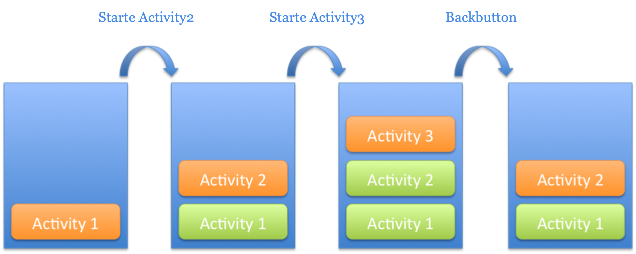
\includegraphics[width=\textwidth]{/backstack.png}
\caption{Back Stack einer Task}
\label{fig:backstack}
\end{figure}

Eine \emph{Task} kann bei entsprechener Benutzer-Interaktion, wie
beispielsweise der Betätigung des \emph{Home-Buttons}, in den Hintergrund treten.
Hierbei werden zwar die enthaltenen Activities gestoppt, der Stack bleibt jedoch intakt.
(vgl. \cite{ADevBackstack})
\subsection{Der Lebenszyklus einer Activity}

\begin{figure}[H]
\centering
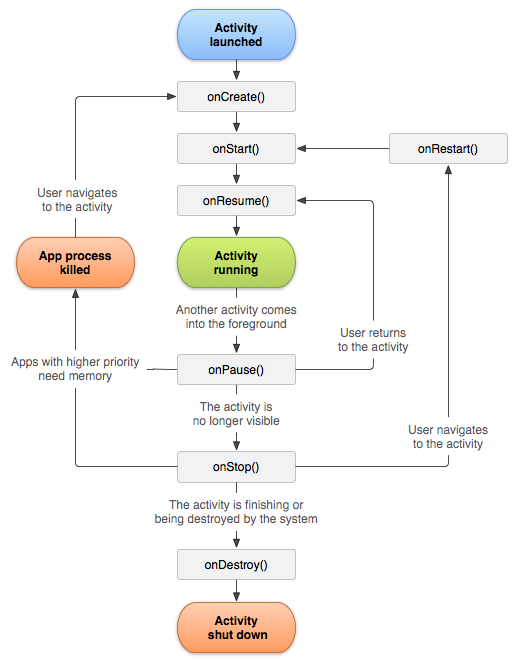
\includegraphics[scale=0.68]{/activity_lifecycle.png}
\caption{Der Activity Lifecycle \cite{ADevActivity}}
\label{fig:actlifecycle}
\end{figure}

Beim Start der Activity werden zunächst der Reihe nach die Methoden \emph{onCreate()},
\emph{onStart()}, \emph{onResume()} aufgerufen. im Anschluß daran läuft die App.

\begin{itemize}
   \item \emph{onCreate()}:\\
   Wird aufgerufen, wenn die Activity zum ersten mal erstellt wird. Infolgedessen ist hier
   der geeignete Ort für Initialisierungen.
   \item \emph{onPause()}:\\
   Diese Methode wird nach Durchlaufen von \emph{onCreate()} aufgerufen, sobald eine andere Activity
   sichtbar wird. Hier sollte der Zustand gesichert werden oder beispielsweise das Abspielen der
   Audiowiedergabe unterbrochen werden.
   \item \emph{onResume()}:\\
   Zum Aufruf von \emph{onResume()} kommt es, falls der Benutzer abermals zu der vorher pausierten
   Activity steuert. Demgemäß sollte hier der vorherige Zustand wieder hergestellt werden.
   \item \emph{onRestart()}:\\
   Wird passiert, falls der Benutzer erneut zu einer gestoppten Activity navigiert, deren
   Speicher nicht benötigt wurde.
\end{itemize}
(vgl. \cite{ADevActivity})   

\subsection{Layouts}
Die visuelle Struktur der Benutzeroberfläche wird normalerweise über XML-Dateien definiert.
Darüberhinaus können die Layouts zur Laufzeit programmatisch durch die Anwendung beschrieben
werden. Da Layout-Dateien mehrfach für eine Activity angelegt werden können, ist es möglich,
verschiedensten Display-Eigenschaften Rechnung zu tragen. Insbesondere können sie an
diverse Displaygrößen angepasst sowie auf Orientierung zugeschnitten werden. Hierfür wird jeweils
ein Ordner mit Namen Layout und entsprechendem Postfix für die gewünschten Eigenschaften erstellt.
In Abbildung \ref{fig:layout_ordner} sind Beispiele für Layout-Ordner dargestellt.

\begin{figure}[H]
\centering
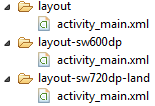
\includegraphics{/layout_ordner.png}
\caption{Layoutdateien für verschiedene Eigenschaften}
\label{fig:layout_ordner}
\end{figure}

Hierbei steht \emph{sw} für die kleinste verfügbare Breite und \emph{land} für die Orientierung
im Querformat. Physikalische Pixel sind je nach Hardware unterschiedlich groß. Um das
Erstellen von Layouts zu erleichtern wurden dichteunabhängige Pixel eingeführt.

\subsubsection*{Density-independent Pixels}
\begin{equation}
pd = px \cdot \frac{160}{dpi}
\end{equation}

\addvspace{2ex}
\textbf{px:} Auflösung in Pixel\\
\textbf{dpi}: Pixeldichte (die Anzahl der Pixel pro Inch)\\

%Demzufolge entsprechen 160 Pixel immer genau einem Zoll.

\subsubsection*{Layout-Arten}

\begin{enumerate}
   \item RelativeLayout:\\
      Die Elemente werden relativ zueinander oder zum Container positioniert.
   \item LinearLayout (horizontal / vertikal):\\
      Ermöglicht eine horizontal oder vertikal aufeinander folgende Anordnung der Elemente 
   \item TableLayout:\\
      Da es sich hierbei um eine tabellenförmige Anordnung handelt, ist es nicht möglich,
      einem einzelnen Element eine eigene Größe zuzuweisen.
   \item GridLayout:\\
      Bei dem mit Android 4. eingeführten Layout werden die Elemente gitterartig positioniert
      Dies bietet mehr Freiheiten bei der Positionierung. Im Gegensatz zum TableLayout können hier
      Elemente unterschiedlich groß sein.
   \item FrameLayout:\\
      Dieses Layout wurde dafür entworfen, einen bestimmten Bereich auf den Bildschirm für ein
      einzelnes Element frei zu halten.
\end{enumerate}
(vgl. \cite{ADevLayout} und \cite{AppsProg}, S. 97)

\subsection{Die Android-Projektstruktur}

\begin{figure}[H]
\centering
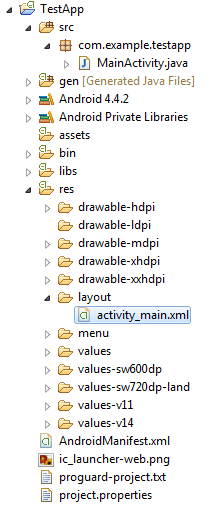
\includegraphics{/android_projektstruktur.png}
\caption{Android Projektstruktur}
\label{fig:android_projektstruktur}
\end{figure}

Die Abbildung \ref{fig:android_projektstruktur} zeigt die Struktur eines neuen, einfachen
Projekts. Eigener Programm-Code befindet sich unterhalb des Ordners \emph{src}.
Alle XML-Ressourcen-Definitionen unterhalb von \emph{res} werden beim Kompilieren in eine
Datei \emph{R.Java} umgewandelt. Dies erspart umständliche Pfadangaben beim Zugriff auf Ressourcen.
Innerhalb der Values-Ordner können zum Beispiel Strings oder Stile festgelegt werden.
Im Android Manifest müssen die Bausteine der App angegeben werden.
Des Weiteren werden dort die Rechte (sog. Permissions, wie beispielsweise der Zugriff
auf bestimmte Informationen) der App aufgeführt.




